\chapter{Relevamiento de aplicaciones de video mapping}
\section{Modul8}
Modul8\cite{Module8} es una herramienta profesional diseñada para realizar espectáculos de video en vivo. Fue creada por VJ's y live performers y esta disponible exclusivamente para plataforma Mac OS mediante licenciamiento propietario.

\begin{figure}[H]
  \centering
    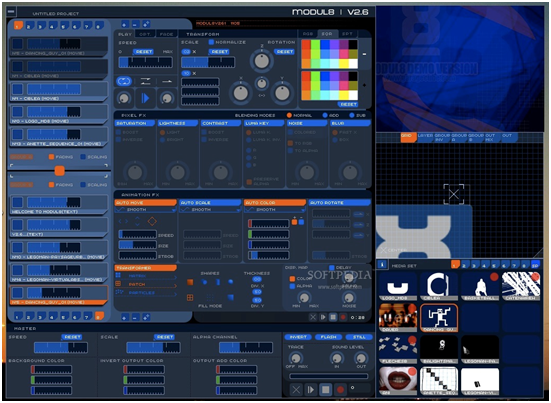
\includegraphics[width=0.6\textwidth]{./Cap3_aplicaciones/apps-modul8.png}
  \caption{Pantalla principal de Module8}
  \label{fig:Apps-Module8}
\end{figure}

La interfaz de usuario está pensada para las performances en vivo, para lo que cuenta con cuatro paneles con funcionalidad bien especifica: un panel principal donde crear y editar las composiciones de video, sonido y efectos; un panel de multimedia manejar los archivos de medios (videos, imágenes, loops de audio, etc); un panel de previsualización donde se puede ir observando la ejecución de una parte de la composición del espectáculo; y por ultimo el panel de salida, donde se observa la composición final que ven los observadores. Todas las funcionalidades provistas pueden ser asignadas a eventos MIDI, por lo que es posible utilizar cualquier dispositivo que los genere para controlar enteramente la aplicación.
Modul8 maneja hasta siete salidas simultaneas de proyección mas otra para la interfaz de usuario. Para hacer uso de esta funcionalidad es necesario contar con una tarjeta de video Pci-Express que de soporte de salida múltiple. Esto activa el modo de salida avanzado dando varias alternativas para la seleccion de la composición o porción de la misma a ser emitida en cada una de las salidas disponibles.
Se maneja el concepto de capa, con un máximo de diez, las que pueden contener sus propios medios, efectos y configuraciones.
Si bien no hay un manejo tridimensional de la escena, la aplicación provee de algunas transformaciones a aplicar a los medios para ajustarlos a la representación bidimensional de los objetos de la escena o incluso a objetos tridimensionales autogenerados que aparecerán en la misma.
La arquitectura de la herramienta permite su extensión mediante la programación de módulos o efectos en el lenguaje Python. En cuanto al rendimiento, se hace un uso intensivo de la unidad de procesamiento gráfica (GPU)\footnote{Ver glosario.} para todo lo que es dibujado, composición y transformaciones de gráficos.
\section{VDMX}
Aplicación para el procesamiento multimedia en tiempo real y disponible exclusivamente para plataforma Mac OS mediante licenciamiento propietario. Es modular y altamente personalizable.

\begin{figure}[H]
  \centering
    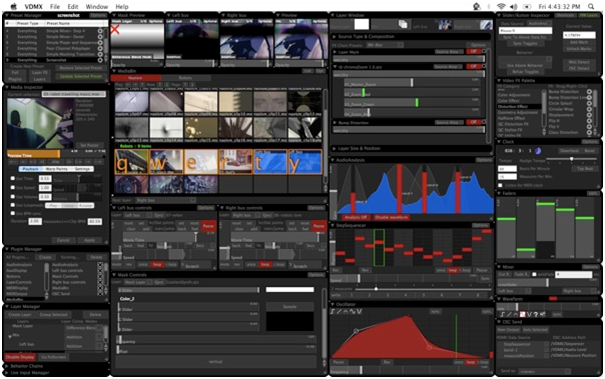
\includegraphics[width=0.6\textwidth]{./Cap3_aplicaciones/apps-vdmx.png}
  \caption{Ejemplo de consola personalizable avanzada realizada en VDMX\cite{VDMX}}
  \label{fig:Apps-VDMX}
\end{figure}


Para ello se provee de funcionalidad básica mediante los llamados Inspectores. El inspector del Grupo de Trabajo expone todo lo que esta sucediendo en VDMX a bajo nivel, como ser los archivos multimedia, las entradas de video configuradas, las capas, los plugins existentes, etc. Luego, el inspector de Interfaz de Usuario permite ver y editar las propiedades de cada control que se selecciona en la interfaz. Adicionalmente, se permite crear interfaces propias a partir de controles básicos como deslizadores, botones, ventanas emergentes, etc, lo que permite a los VJs tener toda la información que crea relevante a disposición en el momento de la representación en vivo.
Se permite asociar eventos de entrada MIDI, OSC o de teclado a cualquier control de la interfaz de usuario, así como también generar eventos MIDI u OSC para ser consumidos por cualquier aplicación externa que los soporte.
Las capas contienen una unica fuente de medios, la que puede ser de tipo video, composición de QuartzComposer o imagen, y adicionalmente se define una cadena de efectos a ser aplicados a la fuente de la capa. La ejecución de la secuencia de efectos puede ser configurada mediante cualquiera de los mecanismos de eventos mencionados anteriormente así como por tiempo (vía plugins). No hay un máximo establecido en el numero de capas que se pueden crear en VDMX, y es posible agruparlas para darle un manejo diferenciado o aplicar efectos a todas a la vez.
Se cuenta con tres modos de salida de video: ventana, pantalla completa y avanzado. En el modo avanzado se permite crear dispositivos de salida, sin un limite predeterminado, y asociarlos a las capas o dispositivos de entrada que se desee.
\section{VVVV}
VVVV\cite{VVVV} es una herramienta que provee un entorno hybrido de programación gráfica y textual de propósito general. Es de uso gratuito para propósitos no comerciales y esta disponible únicamente para plataformas Windows.

\begin{figure}[H]
  \centering
    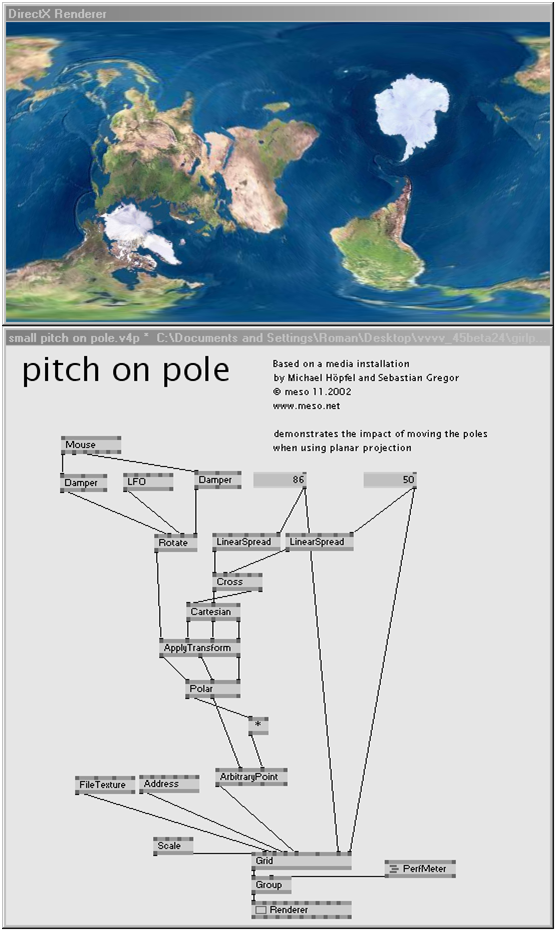
\includegraphics[width=0.5\textwidth]{./Cap3_aplicaciones/apps-vvvv.png}
  \caption{Entorno de programacion de VVVV y salida de video correspondiente}
  \label{fig:Apps-VVVV}
\end{figure}

Para la construcción de un programa se utilizan "Nodos", los que representan operaciones o funciones individuales y los que pueden, eventualmente, tomar una entrada, procesarla, y entregar datos a la salida. Las conexiones entre nodos se llaman "Links" y es como se modela el flujo de información entre nodos. Hay varios tipos de nodos para diferentes propósitos. A modo de ejemplo, el nodo utilizado para desplegar la salida visual del programa es del tipo Renderer, para el agregado de cuadrantes se utiliza el nodo Quad, para el manejo de transformaciones el nodo Transform y para redimensionar a escala el nodo Scale. También hay nodos para cargar objetos tridimensionales, manejar texturas, vectores, temporizadores, etc. Todo en VVVV se representa a través de Nodos.
A diferencia de otros lenguajes de programación, los que cuentas con diferentes modos para construir y ejecutar los programas, VVVV todo el tiempo trabaja en un solo modo, el modo de ejecución, en el que constantemente se están ejecutando cálculos y dibujando gráficos mientras se esta generando o editando un programa.
Para dar soporte multiproyector implementa una arquitectura cliente-servidor, la que permite contar con cualquier cantidad de motores tridimensionales (clientes) manejados desde una instancia de VVVV central (servidor). Toda la configuración y ejecución de un espectaculo distribuido se implementa en un módulo llamado Boygrouping (ref http://vvvv.org/documentation/boygrouping-basics poner foto en http://vvvv.org/documentation/boygrouping-basics).
Se provee soporte para varios protocolos de entrada y salida como TCP, UDP, MIDI y OSC entre otros, y gracias a aportes de la comunidad de programadores VVVV es posible tambien interactuar con dispositivos como Wii, PSP y Kinect. Existen nodos que proveen funcionalidad avanzada como ser soporte para animación y lineas de tiempo, detección y seguimiento de objetos en tiempo real utilizando variadas tecnicas (ARToolkit, OpenCV, etc), emisión de flujos de video, reproducción y mezcla de archivos de audio, simulación de movimiento, colisiones y efectos físicos en general.
El motor gráfico tridimensional de VVVV está basado en Direct3D (referencia), lo que permite hacer un uso intensivo de las placas gráficas modernas para el dibujado de gráficos con alto rendimiento.
VVVV ofrece la posibilidad de crear nodos personalizados a través de una interfaz COM para la implementación de Plugins, lo que ofrece varias alternativas en cuanto a la implementación, pudiéndose utilizar C\#, Delphi o incluso C++.
\section{VPT - Video Projection Tool}
VPT\cite{VPT} es una herramienta para la realización de proyecciones en tiempo real. Es una aplicación de código abierto y de uso y distribución gratuito mediante licenciamiento GNU GPL (referencia). Esta disponible para plataformas Windows y MacOS.

\begin{figure}[H]
  \centering
    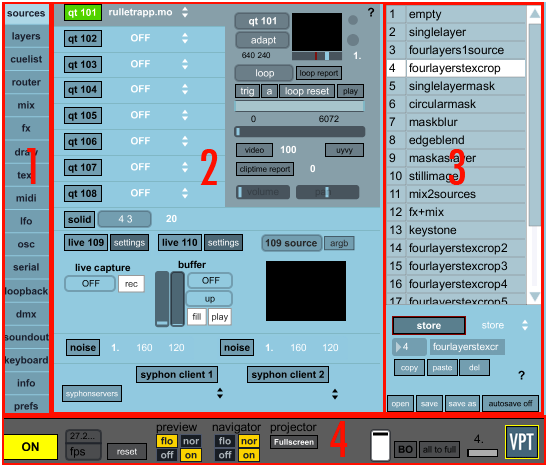
\includegraphics[width=0.65\textwidth]{./Cap3_aplicaciones/apps-vpt.png}
  \caption{Pantalla principal de VPT}
  \label{fig:Apps-VPT}
\end{figure}

La interfaz gráfica es predefinida y cuenta con abundante funcionalidad. Se tiene una barra de herramientas con cada una de las secciones disponibles, las que se muestran en detalle en el panel principal de la aplicación. Siempre disponible a la derecha, están las configruaciones predefinidas. La barra sobre el borde inferior de la pantalla es desde donde se controla la o las salidas de video, la previsualización y otras opciones de navegación.
En cuanto a los posibles orígenes de medios, se puede contar con hasta ocho videos de Quicktime, dos entradas en vivo, las que pueden ser asociadas a cualquier dispositivo de video soportado en el sistema, y una entrada de dibujado en la que es posible crear mascaras personalizadas para objetos sobre los que se proyectara.
Hay una cantidad máxima de 32 capas que se pueden utilizar simultaneamente en un espectáculo. Cada una esta superpuesta sobre la siguiente, y puede ser escalada, posicionada, rotada, distorsionada y enmascarada de manera independiente. También es posible asociarle fuentes de multimedia. Se maneja el concepto de "capa activa" para la edicion y dibujado en la ventana de salida.
Se cuenta con una secuencia de eventos (cuelist) a partir de efectos (presets) almacenados y configurados previamente en el sistema. Para la definición de efectos se cuenta con tipos predefinidos y una nomenclatura para agregarlos a la lista también definida, por ejemplo "F 15 16 5.00" representa un Fade del efecto 15 al 16 con duración 5 segundos, "C 5" ejecuta el efecto numero cinco, "L 3" genera un bucle y vuelve al tercer lugar de la lista de eventos, "D 2" genera una demora de dos segundos y continua con el siguiente evento, etc.

\begin{figure}[H]
  \centering
    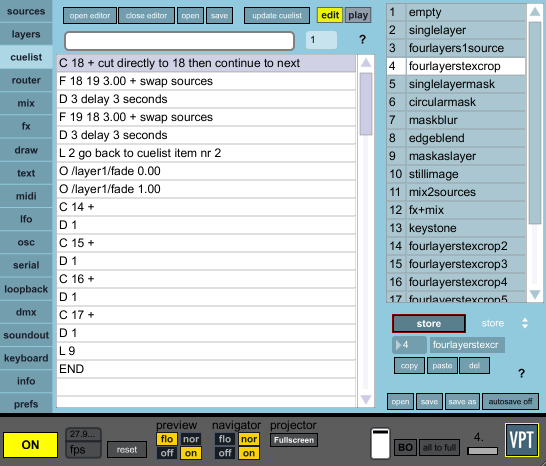
\includegraphics[width=0.65\textwidth]{./Cap3_aplicaciones/apps-vpt-cuelist.png}
  \caption{Efectos y secuencia de eventos de un espectaculo realizado en VPT}
  \label{fig:Apps-VPTCuelist}
\end{figure}

Estando en modo de edición se pueden agregar o eliminar elementos a la lista y estos no serán reflejados en la salida de video aun, mientras que en modo de reproducción constantemente se esta recorriendo al lista de efectos y reproduciendo la salida correspondiente.
Dependiendo de la tarjeta de sonido con la que se cuente, es posible direccionas las entradas de video en hasta 8 canales de salida de audio. El módulo de mezclado permite combinar dos orígenes cualesquiera utilizando diferentes modos. También es posible controlar la aplicación o enviar directamente indicaciones a las capas, orígenes de medios, mezclador, etc, utilizando OSC, MIDI o vía puerto serial con dispositivos como Arduino (http://www.arduino.cc).
Para simular efectos tridimensioanles, se cuenta con la posibilidad de realizar mallas y aplicar asi distorsiones a en una capa dada. Ver aquí un ejemplo de mallas combinado con el uso de MacOS Syphon Recorder (Syphon MacOS Plugin http://syphon.v002.info/). (http://hcgilje.wordpress.com/2011/05/26/vpt-5-5-preview/)
